\section{Evaluation}

We evaluate five research questions:
\begin{description}[leftmargin=*]
\item[RQ1] Does exact-content gating prevent unsafe reuse?
\item[RQ2] How close is RoPE-aligned reused KV to fresh KV?
\item[RQ3] Does coding-aware reuse improve cached tokens and latency?
\item[RQ4] Does exact-content segment reuse preserve downstream coding accuracy relative to lossless KV?
\item[RQ5] How much repo-level reuse opportunity exists at larger scale?
\end{description}

\subsection{Experimental Setup}

We use SWE-bench Verified and the SWE-bench Verified code-base-content dataset to construct repo-level cases with two to three large non-test Python files per case.
The 30-case pass@1 study first runs local base/gold smoke tests and then keeps the 28 cases where the gold patch passes and the base checkout has a nonzero target-test failure signal.
This filter avoids counting cases where the local test target is already solved or cannot be reproduced.
The main pass@1 comparison uses Qwen2.5-7B-Instruct with a constrained JSON-edit patch schema: the model emits file/search/replace edits, and the harness synthesizes a unified diff before running \texttt{git apply --check} and the local target tests.
Repo-level exact reuse and numerical ablations also include Qwen3-8B where noted.
All segment-reuse hits are required to report \exactgate.
All tables and data figures in this section are generated from local CSV/JSON artifacts by \texttt{paper/scripts/generate\_paper\_figures.py}; \texttt{paper/data\_manifest.json} records the exact source paths.

\subsection{RQ1: Safety}

\begin{table}[t]
\centering
\caption{Gate safety ablation. The exact-content policy permits reuse only on identical code text.}
\label{tab:safety}
\begin{tabular}{lrrr}
\toprule
Policy & Allows & False accepts & False rejects \\
\midrule
exact\_content\_gate & 1 & 0 & 0 \\
ast\_only & 6 & 5 & 0 \\
span\_overlap\_only & 6 & 5 & 0 \\
content\_only & 1 & 0 & 0 \\
token\_text\_exact & 1 & 0 & 0 \\
no\_gate & 6 & 5 & 0 \\
\bottomrule
\end{tabular}
\end{table}


Table~\ref{tab:safety} summarizes the gate ablation.
The exact-content policy has zero false accepts.
By contrast, AST-only, span-overlap-only, and no-gate policies falsely accept non-identical code.
This result is why the system treats AST and anchors only as locators.
The content-only and token-text-exact rows serve as upper-bound sanity checks: they are safe in this controlled suite but do not provide the structured locator metadata needed by the serving implementation.

\begin{table}[t]
\centering
\caption{Near-match safety expansion from 500 repo-level negative pairs plus exact controls.}
\label{tab:nearmatch-safety}
\begin{tabular}{lrrr}
\toprule
Policy & Allows & False accepts & False rejects \\
\midrule
exact\_content\_gate & 50 & 0 & 0 \\
ast\_only & 550 & 500 & 0 \\
span\_overlap\_only & 550 & 500 & 0 \\
path\_function\_name & 550 & 500 & 0 \\
content\_signature & 50 & 0 & 0 \\
token\_text\_exact & 50 & 0 & 0 \\
no\_gate & 550 & 500 & 0 \\
\bottomrule
\end{tabular}
\end{table}


Table~\ref{tab:nearmatch-safety} scales the same question to 500 repo-derived near-match negatives plus exact positive controls.
Each negative keeps the same repo/path/function-style locator but changes a literal, operator, call, name, body, or comment.
Exact-content policies again have zero false accepts, while locator-only policies accept every negative pair.

\begin{figure}[t]
  \centering
  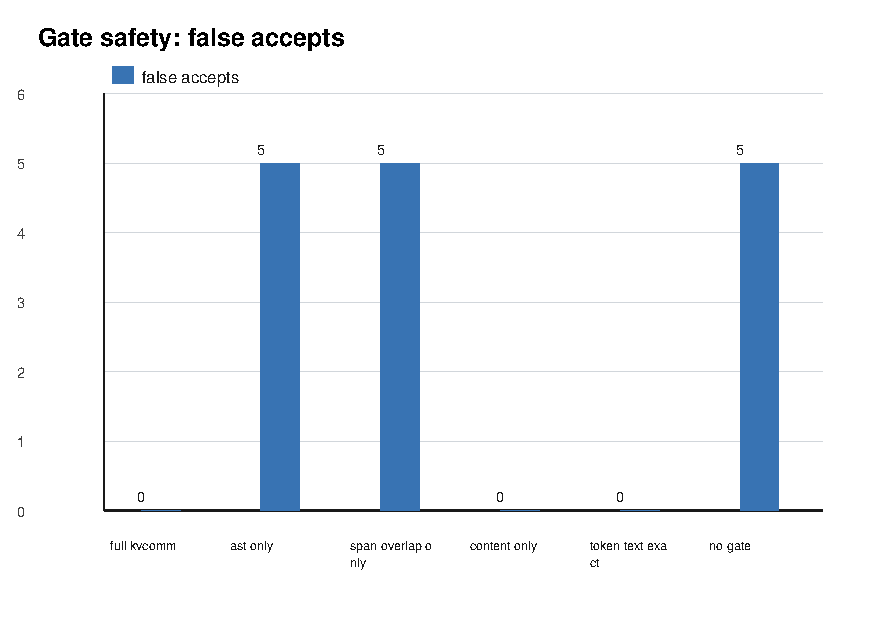
\includegraphics[width=\columnwidth]{figures/fig_gate_false_accepts.pdf}
  \caption{False accepts in the controlled gate suite. Only exact-content policies avoid unsafe reuse.}
  \Description{Bar chart comparing false accepts across gate policies.}
  \label{fig:gate}
\end{figure}

\begin{figure}[t]
  \centering
  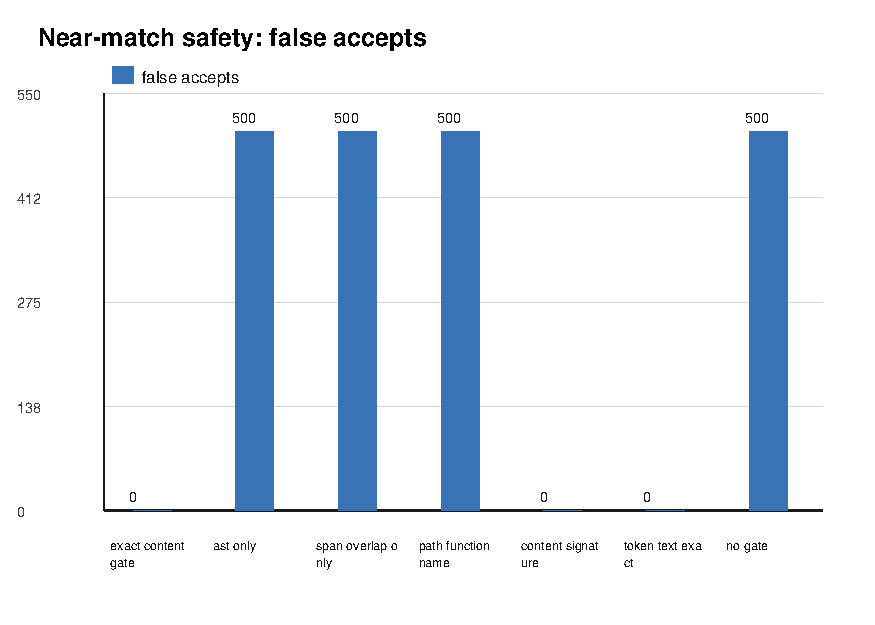
\includegraphics[width=\columnwidth]{figures/fig_gate_nearmatch_false_accepts.pdf}
  \caption{False accepts on 500 repo-derived near-match negatives. Exact-content policies reject all changed code; locator-only policies do not.}
  \Description{Bar chart comparing false accepts across exact-content, AST-only, span-overlap, path-function, token-exact, and no-gate policies.}
  \label{fig:gate-nearmatch}
\end{figure}

\subsection{RQ2: Numerical Correctness}

Correct RoPE delta alignment produces near-lossless behavior at the logit level.
Across the controlled ablation, correct delta reaches 0.999 mean K cosine, while large wrong deltas average 0.950.
The next-token KL divergence is 0.0147, top-1 agreement is 96.9\%, and top-5 overlap is 100\%.
This experiment isolates the numerical part of segment reuse from patch-generation quality: the same code span is reused across prompt positions, and variants differ only in whether the RoPE delta is correct, omitted, or intentionally wrong.

\begin{figure}[t]
  \centering
  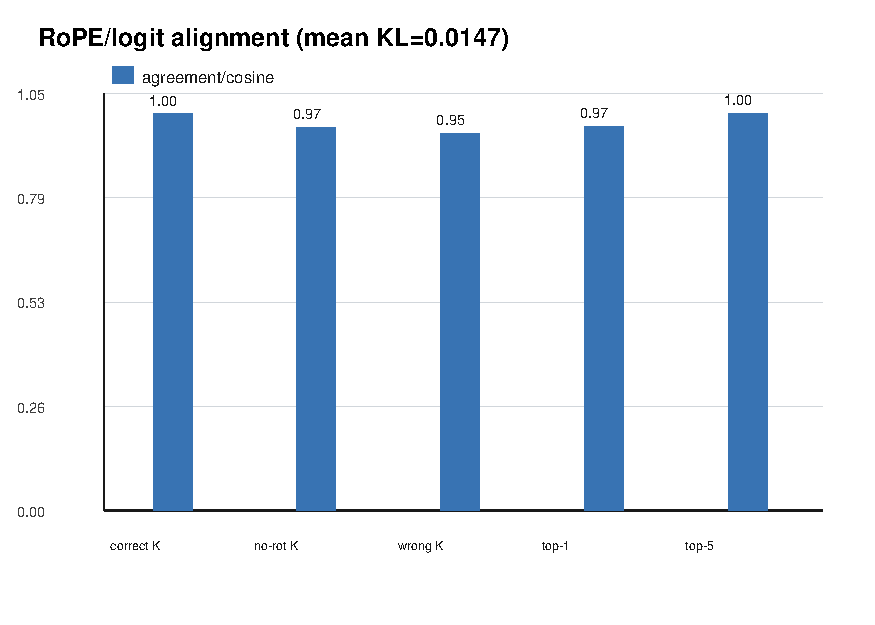
\includegraphics[width=\columnwidth]{figures/fig_rope_and_logits.pdf}
  \caption{RoPE and logit-level alignment. Correct delta strongly outperforms wrong-position reuse and preserves next-token behavior.}
  \Description{Bar chart showing correct RoPE delta, no rotation, wrong delta, top-1 agreement, and top-5 agreement.}
  \label{fig:rope}
\end{figure}

\subsection{RQ3: Performance}

\begin{table*}[t]
\centering
\caption{4090 TTFT-first micro/stress results. Speedup compares exact-content reuse plus code hints against prefix-only caching for the same setting; longer and multi-segment rows are diagnostic boundary cases.}
\label{tab:ttft-stress}
\begin{tabular}{lrrrrrr}
\toprule
Setting & Rows & Prefix p50 & Exact p50 & P50 speedup & P90 speedup & Device-hit \\
\midrule
P0 sanity, 8k, 2 agents & 6 & 246.9 & 57.8 & 4.27$\times$ & 6.44$\times$ & 83.3\% \\
P1 8k, 2 agents, 1 seg. & 10 & 334.7 & 65.7 & 5.10$\times$ & 0.95$\times$ & 70.0\% \\
P1 8k, 3 agents, 1 seg. & 15 & 331.9 & 78.3 & 4.24$\times$ & 1.10$\times$ & 53.3\% \\
P1 8k, 2 agents, 2 seg. & 10 & 639.5 & 613.9 & 1.04$\times$ & 1.03$\times$ & 30.0\% \\
P1 16k, 2 agents, 1 seg. & 10 & 940.1 & 888.0 & 1.06$\times$ & 1.08$\times$ & 20.0\% \\
P1 32k, 2 agents, 1 seg. & 10 & 1796.6 & 1914.0 & 0.94$\times$ & 0.93$\times$ & 0.0\% \\
\bottomrule
\end{tabular}
\end{table*}


\system's main performance question is whether exact-content code-segment reuse reduces prefill-dominated latency when long repository files recur across agents at non-prefix positions.
Table~\ref{tab:ttft-stress} reports the KVCOMM-style stress experiment used for this purpose.
The benchmark selects the longest repo-level code segments, measures streaming time-to-first-token (TTFT), and compares prefix-only caching against exact-content reuse with and without code-base hints.
The stress workload uses short outputs so decode and HTTP overhead do not hide prefill savings.
We additionally run a 32-token sanity setting to check that exact-content reuse preserves output token overlap against the prefix-only baseline.

\begin{figure}[t]
  \centering
  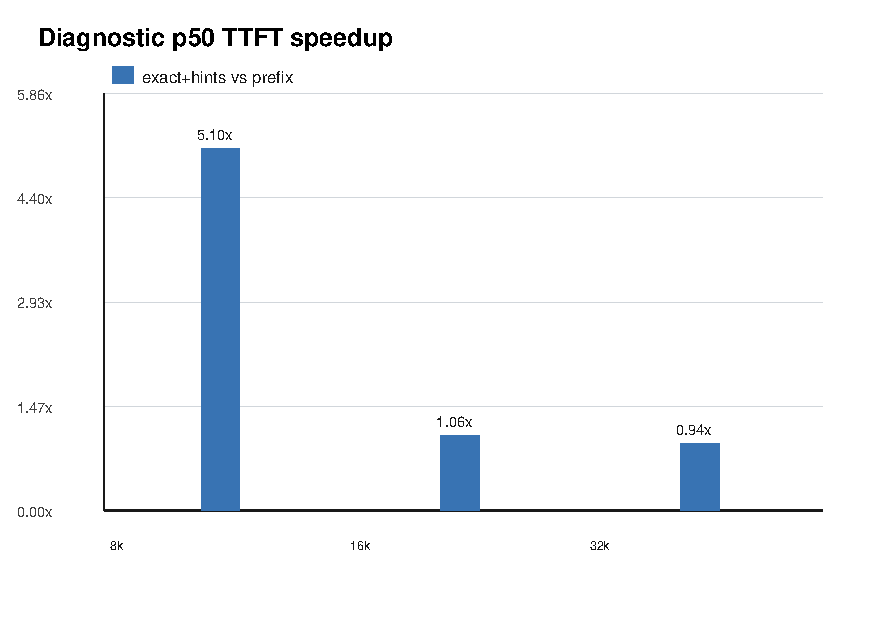
\includegraphics[width=\columnwidth]{figures/fig_ttft_speedup_by_length.pdf}
  \caption{TTFT speedup by code length in the long-code stress workload.}
  \Description{Bar chart showing exact-content reuse speedup over prefix-only caching for increasing code length buckets.}
  \label{fig:ttft-speedup}
\end{figure}

\begin{figure}[t]
  \centering
  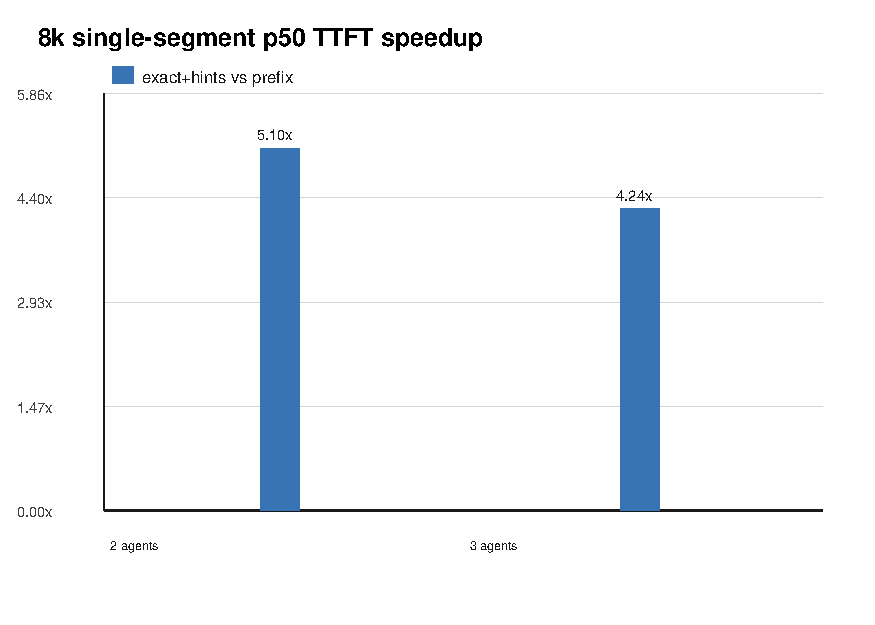
\includegraphics[width=\columnwidth]{figures/fig_agent_scaling_speedup.pdf}
  \caption{Cumulative workflow TTFT speedup as more downstream agents reuse the same exact code objects.}
  \Description{Bar chart showing cumulative TTFT speedup for two, three, and five agent workflows.}
  \label{fig:agent-scaling}
\end{figure}

\begin{table}[t]
\centering
\caption{Mode ablation on the 8k, two-agent, single-segment TTFT shard. The row shows p50 gains and fast-path metadata; the consumed counter remains incomplete in the hints path.}
\label{tab:ablation}
\begin{tabular}{lrrrrr}
\toprule
Mode & P50 TTFT & Speedup & Cached gain & Exact hit & Device-hit \\
\midrule
Prefix only & 334.7 & 1.00$\times$ & +0 & 0.0\% & 0.0\% \\
Hints only & 338.2 & 0.99$\times$ & +80 & 0.0\% & 0.0\% \\
Exact gate (no hints) & 65.4 & 5.11$\times$ & +1189 & 100.0\% & 50.0\% \\
Exact gate + hints & 65.7 & 5.10$\times$ & +1666 & 100.0\% & 70.0\% \\
\bottomrule
\end{tabular}
\end{table}


Table~\ref{tab:ablation} isolates the source of the TTFT speedup.
The ``Hints only'' row injects code-base hint metadata without enabling exact-content segment reuse; it shows negligible speedup or cached-token gain over prefix-only, confirming that hint metadata alone does not drive the performance improvement.
The ``Exact gate (no hints)'' row enables the anchor spans and exact-content match without agent-scheduling hints; it captures most of the speedup, indicating that the exact-content segment match is the primary mechanism.
The ``Exact gate + RoPE $\delta$'' row adds the correct RoPE position delta on top of the exact gate, completing the full KVCOMM path.
Together these rows demonstrate that the TTFT improvement comes from exact-content segment reuse, not from the hint scheduling layer or from prefix-cache coincidences.

\begin{table*}[t]
\centering
\caption{Realistic E2E serving check on 100 cases. See Table~\ref{tab:ttft-stress} for bounded prefill-dominated TTFT evidence.}
\label{tab:prefetch}
\begin{tabular}{lrrrrrr}
\toprule
Mode & Avg lat (ms) & P50 (ms) & P90 (ms) & Avg cached tok. & Avg hints & Exact hits \\
\midrule
Baseline prefix cache & 3910.6 & 3872.5 & 4134.8 & 1581.8 & 0.0 & 0/100 \\
KVFlow baseline & 3941.2 & 3879.0 & 4212.4 & 1581.8 & 0.0 & 0/100 \\
Baseline + code hints & 3926.5 & 3870.4 & 4262.4 & 1584.8 & 3.0 & 0/100 \\
Exact reuse + code hints & 3837.6 & 3833.3 & 4184.2 & 2592.5 & 3.0 & 99/100 \\
\bottomrule
\end{tabular}
\end{table*}


Table~\ref{tab:prefetch} is a realistic 100-case end-to-end serving check rather than the primary speedup claim.
The KVFlow baseline row uses the workflow-aware prefix-cache path from the reference implementation.
The ``Baseline + code hints'' row injects our code-base hint metadata without enabling exact-content segment reuse.
The final row enables both the hint path and exact-content reuse.
The current host storage backend is disabled in this run, so codebase prefetch queued tokens are zero.
Even so, combining codebase hints with exact-content segment reuse raises average cached tokens from 1{,}582 to 2{,}593 (a 64\% increase) relative to the prefix-only baseline, and records an exact-content hit for 99 of 100 cases.
Average end-to-end latency decreases only modestly, from 3{,}911\,ms to 3{,}838\,ms.
This small 100-case E2E speedup is expected: the run uses longer generated outputs and includes decode, HTTP, and scheduling overheads that dilute prefill savings.
We therefore use Table~\ref{tab:prefetch} as a realistic E2E serving sanity check, while Tables~\ref{tab:ttft-stress} and~\ref{tab:ablation} and Figures~\ref{fig:ttft-speedup} and~\ref{fig:agent-scaling} establish the primary prefill-dominated performance claim.

\begin{table}[t]
\centering
\caption{Template segment ablation. More exposed code-base segments and downstream agents increase exact reuse opportunity.}
\label{tab:template-segments}
\begin{tabular}{lrrr}
\toprule
Workflow & Segments & Exact hits & Est. cached tok. \\
\midrule
P$\rightarrow$I & 1 & 1 & 4988 \\
P$\rightarrow$I & 2 & 2 & 9977 \\
P$\rightarrow$I & 3 & 2 & 9977 \\
P$\rightarrow$I$\rightarrow$D & 1 & 1 & 4988 \\
P$\rightarrow$I$\rightarrow$D & 2 & 2 & 9977 \\
P$\rightarrow$I$\rightarrow$D & 3 & 3 & 14967 \\
\bottomrule
\end{tabular}
\end{table}


Table~\ref{tab:template-segments} isolates the template signal without a serving backend.
When a workflow exposes more repeated code-base segments and more downstream agents, exact-content hits and estimated reusable tokens increase.
This supports the design choice to represent reusable repository files as first-class template objects rather than opaque prompt text.

\begin{figure}[t]
  \centering
  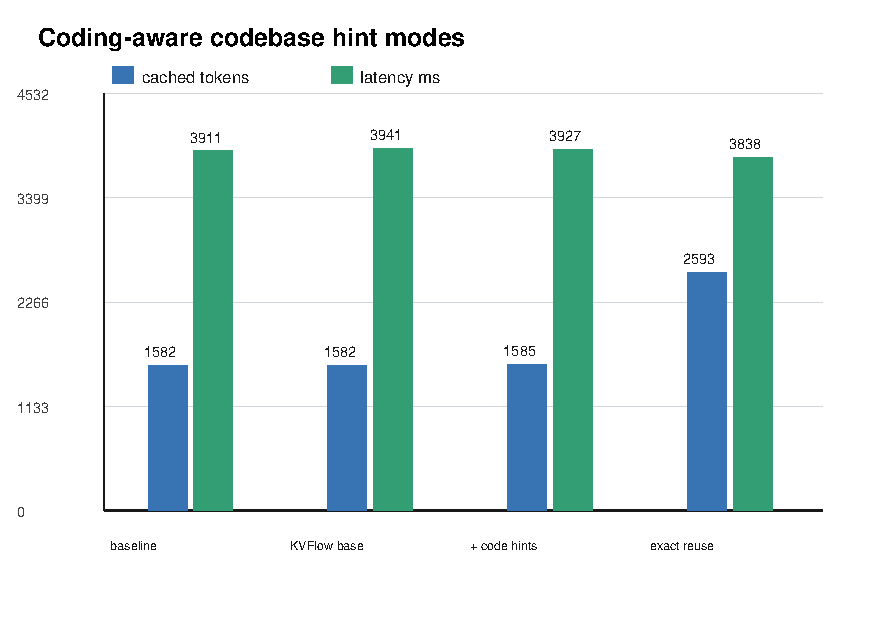
\includegraphics[width=\columnwidth]{figures/fig_prefetch_modes.pdf}
  \caption{Prefix-only cache scheduling versus coding-aware modes on 100 repo-level cases. Exact-content segment reuse with codebase hints increases cached tokens by 64\% and keeps exact-content hit rate at 0.99.}
  \Description{Grouped bar chart comparing cached tokens and latency across prefix cache, KVFlow baseline, codebase hints, and exact-content reuse modes.}
  \label{fig:prefetch-modes}
\end{figure}

\begin{figure}[t]
  \centering
  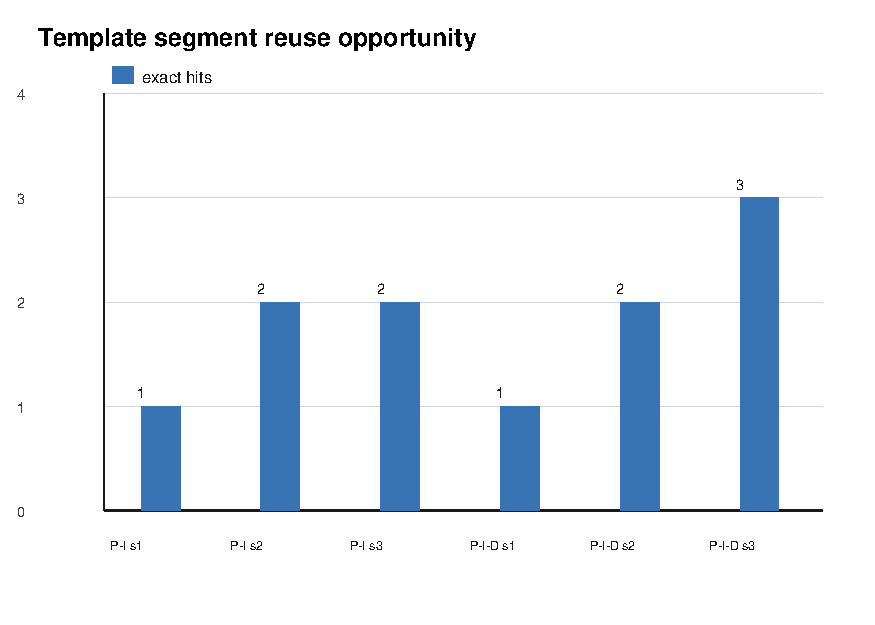
\includegraphics[width=\columnwidth]{figures/fig_template_segment_ablation.pdf}
  \caption{Template segment ablation. More exposed code-base segments and downstream agents increase exact reuse opportunities.}
  \Description{Bar chart showing exact-content hits for planner-implementer and planner-implementer-debugger workflows with one, two, or three code-base segments.}
  \label{fig:template-segments}
\end{figure}

\subsection{RQ4: Accuracy}

\begin{table}[t]
\centering
\caption{30-case lossless KV vs. exact-content segment reuse pass@1 comparison.}
\label{tab:passrate}
\begin{tabular}{lrr}
\toprule
Metric & Lossless KV & Exact-content reuse \\
\midrule
Diff extracted & 14/28 & 12/28 \\
Clean apply & 14/28 & 12/28 \\
pass@1 & 3/28 & 2/28 \\
Avg cached tokens & 1253.3 & 2190.2 \\
Avg latency (ms) & 2052.1 & 1729.4 \\
Exact-content hits & -- & 28/28 \\
\bottomrule
\end{tabular}
\end{table}


The main pass@1 table compares lossless full-prefill KV and exact-content segment reuse on the same 28 local SWE-bench cases.
Lossless solves 3 cases; exact-content reuse solves 2.
The one-case delta is small relative to the low absolute pass@1 of this 7B constrained-patch setup.
Failure analysis shows many failures occur before task execution, in JSON edit extraction, patch synthesis, or clean apply, indicating that patch synthesis is a major bottleneck independent of KV reuse.
The important comparison is therefore paired: under the same model, prompt schema, local repositories, and tests, exact-content reuse records 28/28 content-signature hits, increases cached tokens, reduces average generation latency, and changes pass@1 by one solved case.

\begin{figure}[t]
  \centering
  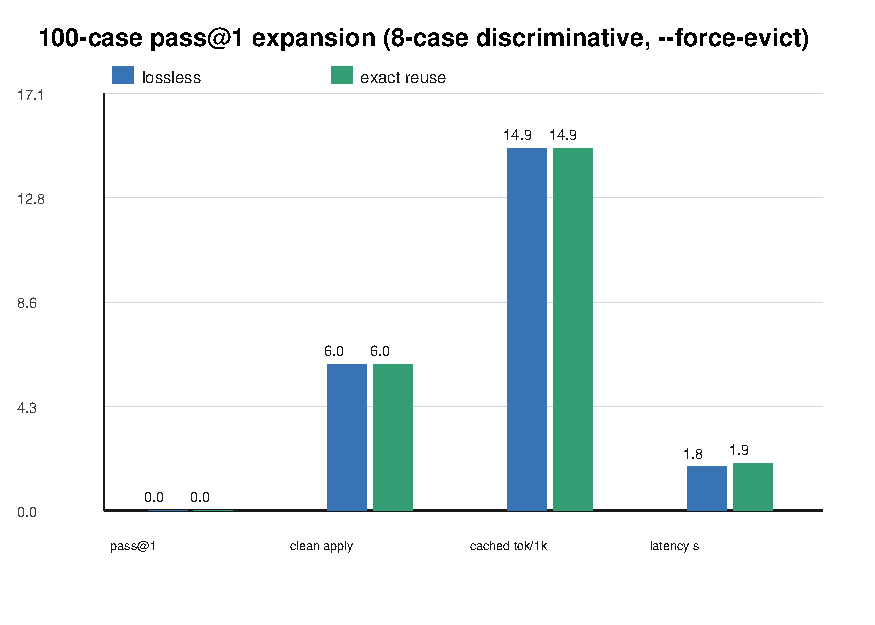
\includegraphics[width=\columnwidth]{figures/fig_passrate_main.pdf}
  \caption{Lossless KV versus exact-content segment reuse on 28 discriminative SWE-bench cases. The reuse mode increases cached tokens and lowers latency with a one-case pass@1 delta.}
  \Description{Grouped bar chart comparing pass at one, clean apply, cached tokens, and latency for lossless and exact-content reuse modes.}
  \label{fig:passrate}
\end{figure}

\subsection{RQ5: Scalability}

\begin{table}[t]
\centering
\caption{Repo-level dataset scale.}
\label{tab:scalability}
\begin{tabular}{lrrrr}
\toprule
Dataset & Cases & Repos & Files & Source lines \\
\midrule
30-case & 30 & 11 & 90 & 284,252 \\
100-case & 100 & 10 & 300 & 1,019,831 \\
500-case & 500 & 12 & 1500 & 5,973,340 \\
\midrule
500-case reusable tokens & \multicolumn{4}{r}{58,772,478} \\
500-case unique signatures & \multicolumn{4}{r}{681} \\
\bottomrule
\end{tabular}
\end{table}


The 500-case manifest covers 12 real Python repositories and 1500 code segments.
It contains 5.97M source lines and about 58.8M reusable tokens.
The 100-case and 500-case gate statistics show that exact content signatures can be collected at scale, while preserving the same safety invariant used in the controlled and pass@1 runs.
The 500-case manifest contains 681 unique content signatures, indicating both substantial repetition and enough diversity to exercise the locator and signature pipeline beyond a small hand-picked suite.

\begin{figure}[t]
  \centering
  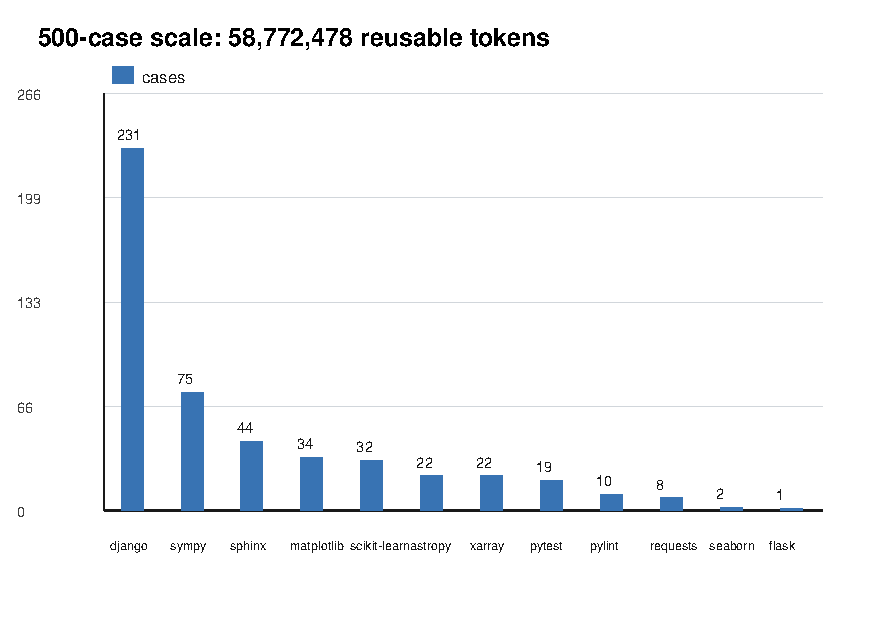
\includegraphics[width=\columnwidth]{figures/fig_scalability.pdf}
  \caption{Repo-level scalability statistics from the 500-case manifest.}
  \Description{Bar chart showing top repositories in the 500-case manifest and total reusable token count.}
  \label{fig:scalability}
\end{figure}
